\documentclass[../main.tex]{subfiles}
\graphicspath{
    {"../img/"}
    {"img/"}
}

\begin{document}
\[
    \varepsilon = min \left\{ |t_0-a|,|t_0-b|,\frac{1}{L},\frac{r_2}{M} \right\}
\]
\[
    ]t_0-\varepsilon,t_0+\varepsilon[
\]
Chcielibyśmy, żeby $\varepsilon$ nie zależał od punktu w którym zaczniemy.\\
Zauważmy, że
\[
    \Vert  A(t)x(t)+b(t)  \Vert \le L(\Vert x_0\Vert +r_2 ) +c
\]
zatem
\begin{align*}
    &\frac{r_2}{M} \ge \frac{r_2}{L(\Vert x_0 \Vert +r_2)+c}= \Bigg| \text{Połóżmy }r_2 = \Vert x_0 \Vert +c \Bigg| =\\
    &= \frac{\Vert x_0 \Vert +c}{L(\Vert x_0 \Vert +\Vert x_0 \Vert +c)+c}=\\
    &\frac{\Vert x_0 \Vert +c}{L(2\Vert x_0 \Vert +c)+c}\ge \frac{\Vert x_0 \Vert +c}{L(2\Vert x_0 \Vert +c+c) + c + \Vert x_0 \Vert } = \\
    &\frac{1}{2L+1},
\end{align*}
zatem
\[
    \varepsilon = min \left\{ |t_0-a|,|t_0-b|,\frac{1}{L},\frac{1}{2L+1} \right\}
\]
($r_1$ - pomijamy, bo $A(t)$ -  ciągła na $[a,b]$).\\
Oznacza to, że wartość $\varepsilon$ nie zależy od $x$, zatem rozwiązanie początkowo określone na
\[
    ]t_0-\varepsilon,t_0+\varepsilon[ \times K(x_0,r_2)
\]
możemy przedłużyć do określonego na całym $[a,b] \times X$ !

    \subsection{Rezolwenta}
    Rozwiązaniem problemu Cauchy
    \begin{align*}
        &\frac{dx}{dt} = A(t)x(t)+b(t)\\
        &x(t_0)=x_0
    .\end{align*}
    jest funkcja $x(t,t_0,x_0)$
\begin{figure}
    \centering
    \includegraphics[width=0.8\textwidth]{fig_31}
    \caption{Mała zmiana może dać rozwiązanie w podobnym miejscu ale nie musi}
    \label{fig:fig_31}
\end{figure}

\begin{pytanie}
    Czy istnieje
    \[
        R(t,t_0): \mathbb{R}^n\to\mathbb{R}^n
    .\] Takie, że
    \[
        x(t) = R(t,t_0)x_0?
    .\](Jeżeli $x_0,x(t)\in\mathbb{R}^n$)
\end{pytanie}

\begin{figure}
    \centering
    \includegraphics[width=0.8\textwidth]{fig_32}
    \caption{Jak pośpimy minutę dłużej to nic się nie stanie (świat jest ciągły)}
    \label{fig:fig_32}
\end{figure}

\begin{definicja}
    Jakie własności $R(t,t_0)$ powinno posiadać?
    \begin{enumerate}
        \item $R(t,t_0): \mathbb{R}^n\to\mathbb{R}^n, R$ - liniowy\label{eq:131}\\
            Bo jeżeli $x_1(t), x_1(t_0)=x_0^1$ i $x_2(t),x_2(t_0) = x_0^2$ są rozwiązaniem, to chcielibyśmy, by  $x_1(t) + x_2(t)$ też było rozwiązaniem z wartością początkową $x_0^1+x_0^2$. Rys \ref{fig:fig_32}
        \item funkcja $R(t,t_0)$
        \item $R(t,t_0) = R(t,s) R(s,t_0)$\\
            $\underset{t,t_0,s\in\mathcal{O}\subset\mathbb{R}}{\forall} $
        \item $R(t_0,t_0) = \mathbb{I}$, bo $x(t) = R(t,t_0)x_0$
            $\underset{t_0\in\mathcal{O}}{\forall} $ \\
            Ad 3. Wstawiając $t_0$ do trzeciej kropki otrzymujemy
            \[
                R(t_0,t_0)=R(t_0,s)R(s,t_0)\rightarrow \underset{t,s\in\mathcal{O}}{\forall} R(s,t) = R(t,s)^{-1}
            \]
        \item
            \begin{align*}
                &\frac{dR(t,to)}{dt} = A(t)R(t,t_0),\\
                &R(t_0,t_0) = \mathbb{I}
            .\end{align*}
            bo wtedy
            $x(t) = R(t,t_0)x_0$ jest rozwiązaniem problemu
            \begin{align*}
                &\frac{dx}{dt}=A(t)x(t)\\
                &x(t_0)=x_0
            .\end{align*}
            bo $\frac{dx}{dt} = \frac{d}{dt}(R(t,t_0)x_0) = A(t)R(t,t_0)x_0=A(t)x(t)$ i $x(t_0)=R(t_0,t_0)x_0 = \mathbb{I}x_0 = x_0$
    \end{enumerate}
\end{definicja}

    Zatem na mocy twierdzenia o jednoznaczności rozwiązań wiemy, że założenie $x(t) = R(t,t_0)x_0$ da nam jednoznaczne rozwiązanie.
    \begin{pytanie}
        A co z $b(t)$? (ten wektorek co by to był, ale go nie ma)
    \end{pytanie}
    Chcemy rozwiązać problem
    \begin{align*}
        &\frac{dx}{dt}=A(t)x(t)+b(t)\\
        &x(t_0)=x_0
    .\end{align*}
    Załóżmy, że rozwiązanie tego problemu możemy przedstawić jako
    \[
        x(t) = R(t,t_0)C(t), C(t):\mathbb{R}\to\mathbb{R}^n
    .\]
    Ale
    \[
        \frac{d}{dt}x(t) = \frac{d}{dt} \left( R(t,t_0)c(t) \right) = \frac{dR(t,t_0)}{dt}c(t)+R(t,t_0)\frac{dc}{dt} = A(t)R(t,t_0)c(t_)+R(t,t_0)\frac{dc}{dt}
    .\]
    Zatem mogę napisać, że
    \[
        A(t)R(t,to)c(t)+R(t,t_0)\frac{dc}{dt}=A(t)R(t,t_0)c(t)+b(t)
    .\](cudowne skrócenie)
    \[
        R(t,t_0)\frac{dc}{dt}=b(t) \quad\quad/R(t,t_0)^{-1}
    .\]
    \[
        \frac{dc}{dt}=R(t,t_0)^{-1}b(t)
    .\]
    \[
        \frac{dc}{dt} = R(t,t_0)b(t)
    .\]
    \[
        c(t) -\alpha = \int_{t_0}^t R(t_0,s)b(s) ds, \alpha\in\mathbb{R}
    .\]
    Ale $c(t_0)=x_0$, więc $\alpha = x_0$.
    \[
        c(t) = x_0+\int_{t_0}^t R(t_0,s)b(s)ds
    .\]
    Zatem
    \[
        x(t) = R(t,t_0)c(t) = R(t,t_0)\left( x_0+\int_{t_0}^t R(t_0,s)b(s)ds \right)  =
    .\]
    \[
        R(t,t_0)x_0+R(t,t_0)\int_{t_0}^t R(t_0,s)b(s)ds =
    .\]
    \[
        R(t,t_0)x_0+\int_{t_0}^t \underset{R(t,s)}{R(t,t_0)R(t_0,s)}b(s)ds
    .\]
    Zatem rozwiązanie problemu wygląda tak:
    \[
        x(t) = R(t,t_0)x_0+\int_{t_0}^t R(t,s)b(s)ds
    .\]
    dygresja:\\
    dają nam rozkład gęstości masy $\rho(x')$. Jak wygląda potencjał?
     \[
         \varphi(x) = \int \frac{\rho(x') dv'}{\Vert x-x' \Vert }
    .\]
    W tym przypadku rezolwenta to $\frac{1}{\Vert x-x' \Vert }$\\

    \begin{pytanie}
        Czy rezolwenta istnieje?
    \end{pytanie}
    Funkcja $R(t,t_0) = e^{\int_{t_0}^t A(s) ds}$ spełnia warunki $1-5$ dla rezolwenty
    \begin{itemize}
        \item $R(t,t_0): \mathbb{R}^n\to\mathbb{R}^n$
        \item $R(t,t_0)$ - jest ciągła względem $t$ i $t_0$
        \item $R(t,\alpha)R(\alpha,t_0) = R(t,t_0)$, bo $e^{\int_{t_0}^t A(s)d s} = e^{\int_{t_0}^\alpha A(s)d s+\int_{\alpha}^t A(s)d s}$\\
            $R(t,t_0) = R(t,\alpha)R(\alpha,t_0)$
        \item $R(t_0,t_0) = e^{\int_{t_0}^{t_0}A(s)d s} = \mathbb{I}$
        \item $\frac{dR}{dt}=A(t)R(t,t_0)$\\
            Dowód:
            \[
                \frac{R(t+h,t_0) -R(t,t_0)}{h} = \frac{1}{h}\left(e^{\int_{t_0}^{t+h}A(s)d s} - e^{\int_{t_0}^{t}A(s)d s}\right) =
            .\]
            \[
                =\frac{1}{h}\left[ e^{\int_{t_0}^{t+h}A(s)d s}e^{\int_{t_0}^{t}A(s)d s}-e^{\int_{t_0}^{t}A(s)d s} \right] =
            .\]
            \[
                \frac{1}{h}\left[ e^{\int_{t}^{t+h}A(s)d s}-\mathbb{I} \right] e^{\int_{t_0}^t A(s)d s} - \frac{1}{h}\left[ e^{hA(\beta) - \mathbb{I}} \right] R(t,t_0) =
            .\]
            \[
                \frac{1}{h}\left[ \mathbb{I}+\frac{hA(\beta)}{1} + \frac{(hA(\beta))^2}{2!}+\ldots = \mathbb{I} \right] R(t,t_0) =
            .\]
            \[
                \underset{t<\beta<t+h}{A(\beta)R(t,t_0)} + h[...]\to A(t)R(t,t_0)
            .\]
            (((($\int_{t}^{t+h}A(s)d s = (t+h-t)A(\beta)$))))
    \end{itemize}
    \begin{przyklad}
        \[
            \frac{d}{dt}\begin{bmatrix} x(t)\\p(t) \end{bmatrix}  = \begin{bmatrix} 1&0\\0&-1 \end{bmatrix} \begin{bmatrix} x(t)\\p(t) \end{bmatrix} , \begin{bmatrix} x(0)\\p(0) \end{bmatrix} = \begin{bmatrix} x_0\\p_0 \end{bmatrix}
        .\]
        \[
            \begin{bmatrix} x(t)\\p(t) \end{bmatrix} e^{\int_{0}^t \begin{bmatrix} 1&0\\0&-1 \end{bmatrix} ds}\begin{bmatrix} x_0\\p_0 \end{bmatrix} = e^{t\begin{bmatrix} 1&0\\0&-1 \end{bmatrix} }\begin{bmatrix} x_0\\p_0 \end{bmatrix}
        .\]
    \end{przyklad}
\end{document}
